\chapter{Preliminaries}\label{chapter:background}

To embed this thesis into existing work, we will first give a short introduction to the field of neural networks and XAI. This will be followed by a more in-depth look at layer-wise- and concept relevance propagation which is to be evaluated in our analysis. Previous work on evaluation of XAI, which is related to our analysis, is followed by the introduction of the main ideas of the causality framework we are going to use for our evaluation experiment. 

\section{Neural Networks}
Among the many machine learning approaches that have been developed, the most popular, but arguably most opaque, are deep neural networks. In general, a neural network consists of neurons, which are computational nodes organized in layers. In the most simple forward pass, each neuron weighs its inputs, offsets them with a bias and then feeds the result through a non-linear function. This is repeated in the next layer of neurons until the output layer is reached. During training, a loss function between the predictions for data instances and their true labels is optimized by back-propagating its gradient and updating the internal weights and biases. For specifics on successful architectures and training procedures we refer to text books on deep learning, for example by \cite{Goodfellow2016}. When trained with enough data, the weights and biases together approximate a high-dimensional and non-linear function describing the training data. This function however is hard to analyze and interpret for humans when trying to understand the reasoning of the network. This lead to the emergence of many explanation methods attempting to uncover those inner workings in a human-interpretable way.


\section{Explainable Artificial Intelligence}
With the field of machine learning and particularly complex deep neural network models continuously expanding, so is the demand for explanations of these models.
As especially neural networks are so called \textit{black boxes} that inhibit a human understanding of their results, plenty of explanation methods have been developed, summarized under the acronym XAI. The sub-field of interpretable AI aims to create inherently transparent models, but they may come with a decrease in performance \cite{Lipton2018}. Therefore, many XAI methods are explaining what a model has learned \textit{post-hoc}, either model-agnostic by only evaluating decisions based on input data or model-specific by using information on latent parameters of a model.

Post-hoc methods can be generally divided into local and global approaches. Local methods aim to explain the decision making for one specific example, like one image in a computer vision task, typically by attributing importance to input features. 
These methods applied to compute vision tasks, are also called saliency map methods and assign importance to pixels or regions of a sample image, creating a heatmap. 
The importance is either computed through forms of back-propagation \citep{Bach2015,Zhang2016,Kindermans2017}, with the help of the model's gradients \citep{Sundararajan2017,Smilkov2017}, or in a model-agnostic way by perturbing or occluding parts of the input \citep{Lundberg2017,Zeiler2013,Zintgraf2017,Agarwal2020}. Resulting saliency maps may generate insight into the locality of important objects. However, this is usually only one facet of understanding the decision-making of a model, especially for people not familiar with the data domain. If the location of importance is identified, it is still not clear what is important in that area.   

Global methods, on the other hand, yield more general interpretations of a model, for example, which abstract features are identified in the decision-making process or how they interplay. An example is activation-maximization \cite{Nguyen2016} which finds prototypical instances with maximal activation for a class. 

Recently, there has been a surge in connecting such global methods with local methods, e.g., by embedding saliency maps into the more global strategy of a model. \cite{Achtibat2022} use an adapted local attribution method to aid in finding human-interpretable abstract concepts that a model encodes. As a back-propagation method their approach utilizes the space of latent layers of a neural network to find abstract components in the input space encoded within the model. The aim to find and quantify the importance of an abstract concept is shared by a growing set of concept-based methods \citep{Bau2017,Bau2020,Kim2018, Ghorbani2019, Zhang2021, Fel2023a}. 
Some approaches are partly supervised, in that a human has to first define what a concept is, e.g. by labelling a ground truth dataset or by selecting a few images that belong to a certain concept \citep{Kim2018, Singla2022}. Others try to make sense of either the latent space spanned by the \textit{concept activation vectors} or the space of per-pixel attributions, for example, by clustering it \citep{Lapuschkin2019,Vielhaben2023} and disentangling and visualizing concepts  \citep{Ghorbani2019,Zhang2021,Leemann2023,Fel2023,Chormai2022, Singla2022}.


\subsection{Layer-wise Relevance Propagation}\label{section:lrp}
Layer-wise Relevance Propagation (LRP) \citep{Bach2015} is the basis for Concept Relevance Propagation (CRP), which we will analyze in this thesis, and is among the most highly cited local attribution methods in XAI. Having been introduced almost 10 years ago, it has been justified mathematically with Deep Taylor Decomposition \citep{Montavon2017}. It belongs to the class of (modified) back-propagation methods which propagate a custom value back to the input through a set of backpropagation rules. A visual representation of this strategy can be found in \cref{fig:crp_vs_lrp} \textbf{(a)}. Like other saliency methods, LRP is commonly used in computer vision tasks to attribute importance to each pixel in an image, which can then be visualized as a heatmap, but is also applicable to other data formats. In the following we will summarize the basic functioning of LRP for neural networks as described by \cite{Bach2015}:

The general idea is to find how input features contribute to a prediction in relation to a root point of maximal uncertainty $f(\mathrm{x}_0) = 0$ so that the positive or negative relevances $R_d \in \mathbb{R}$ of separate input features $d$ for instance $\mathrm{x} \in \mathbb{R}^D$, e.g., pixels, roughly sum up to the output for the model $f$:
\begin{equation}\displaystyle
    f(\mathrm{x}) \approx \sum_{d=1}^{D} R_d
\end{equation}

LRP assumes that the model has multiple layers of computation ($\ell \in L$) it can be decomposed into, starting from the input layer, for example the pixels of an image, to all latent layers and finally to the output layer. Further, each of those layers has $|\ell|$ dimensions for which a relevance score $R^{\ell}_d$ can be determined so that the following equation holds, which constitutes the conservation of total relevance between layers:
\begin{equation}
    f(\mathrm{x}) = ... = \sum_{d \in \ell+1} R^{(\ell+1)}_d =  \sum_{d \in \ell} R^{(\ell)}_d = ... =  \sum_{d} R^{(1)}_d
\end{equation}

In neural networks, the general forward step for a layer $j$ means weighing the previous layer's $i$ outputs $f_i(\mathrm{x})$ with the current layer's weights $z_{ij} = f_i(\mathrm{x}) w_{ij}$, summing the results for all connected neurons and their bias $z_{j} = \sum_{i} z_{ij} + b_j$ and running this through a non-linear activation function $f_j(\mathrm{x}) = \sigma (z_j)$.
The intuition then is to follow the flow of relevance from the output, where usually the prediction value $f(\mathrm{x})$ is taken to initialize the relevance, back to the input layer by decomposition. In the simplest case relevance is propagated back proportionally to the weights to the previous layer where the relevance of all connected neurons is aggregated by a weighted sum:
\begin{equation}\label{eq:basic_attribution_rule}
    R_i = \sum_{j}  R_{i \leftarrow j} = \sum_{j} \frac{z_{ij}}{z_j} R_j
\end{equation}

To apply LRP, certain best practices and rules have been established \citep{Kohlbrenner2020, Montavon2019, Samek2021}. Depending on the type and location of a layer within a neural network the propagation rule can be varied. In this thesis we stick to the method that the authors of CRP use, namely the composite $LRP_{\varepsilon-z+-\flat}$-rule (read ``epsilon-plus-flat''), which is recommended by \cite{Kohlbrenner2020} and composes different rules for different parts of the model, further described in the \cref{appendix:lrprules}.

\subsection{Concept Relevance Propagation}\label{section:crp_background}
Concept Relevance Propagation (CRP), a recent contribution by \cite{Achtibat2022}, is called a \textit{glocal} XAI method by its authors, extending on the established local attribution technique LRP \cite{Bach2015} and applying other more global methods like \textit{relevance maximization}. 
Layerwise Relevance Propagation, as a local XAI method, produces saliency maps for single data samples through a modified backpropagation process as described in the previous section. By filtering on subsets of latent features within the layers of the model during this modified backpropagation, CRP yields saliency maps which could, in principle, produce more targeted explanations. This is, if the assumption holds that the concepts encoded by latent neurons are representing disentangled features which can be attributed to in varying degrees. With the help of feature visualization methods CRP's authors try to go beyond the pure ``where'' of saliency maps, towards a ``what'', explaining which abstract and possibly human-interpretable concepts a model has recognized in a specific image region. This idea is integrating into the mentioned growing field of \textit{concept-based} explanation methods.

\begin{figure}[t!]
    \centering
    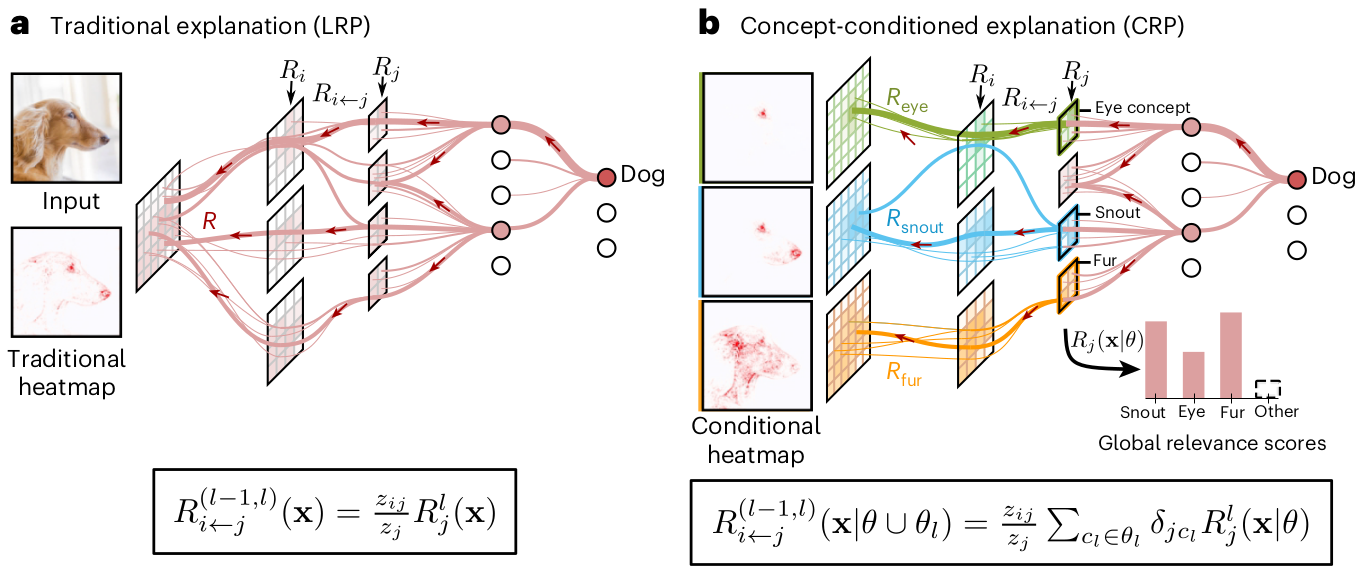
\includegraphics[width=0.9\textwidth]{thesis_latex_template/pics/crp_vs_lrp_from_paper.png}
    \caption[CRP vs. LRP]{\textbf{a} (LRP): output value back-propagated through network, \textbf{b} (CRP): output conditioned on concepts, i.e., certain neurons are masked out in back-propagation (taken from \cite{Achtibat2023}'s more recent paper summarizing Concept-Relevance Propagation)}
    \label{fig:crp_vs_lrp}
\end{figure}

LRP aggregates the significance of all latent layers and their neurons into one importance map, where the intermediate layers' outputs are merely a side-product of the computation.
\cite{Achtibat2022} propose in their work to use those intermediate results to make the attributions concept-specific. In LRP the initialization at the output layer usually takes the value of one class output $y= f(\mathrm{x})$ w.r.t input $\mathrm{x}$, all other output neurons set to zero, and thereby produces a class-conditional attribution ($R(\mathrm{x}|y)$). A similar thing can be done in latent layers too. Although it is yet unclear how to interpret the attribution to these hidden features, the authors of CRP propose to obtain importance scores for them by computing \textit{(multi-)concept-conditional} relevances $R(\mathrm{x}|\theta)$. The variable $\theta$ here describes a set of conditions $c$ which in essence filters for certain ``concepts'' (neurons) in potentially multiple layers by masking out all other neurons' contributions:

\begin{equation}\displaystyle
    R^{(\ell-1, \ell)}_{i \leftarrow j} (\mathrm{x} | \theta \cup \theta_{\ell}) = \frac{z_{ij}}{z_j} \cdot \sum_{c_{\ell} \in \theta_{\ell}} \delta_{jc_{\ell}} \cdot R^{\ell}_j (\mathrm{x} | \theta )
\end{equation}

Here, $\delta_{jc_{\ell}}$ is the Kronecker-Delta selecting the relevance $R^l_j$ of feature $j$ in layer $\ell$ if that index is in the condition $c_{\ell}$ of a layer, masking out all other features in that layer. If no condition is set for a particular layer, the relevance from that layer is not masked. The authors note that conditions compare to logical OR operations within the same layer and to AND operations across layers. 

\subsubsection{Interpretation Techniques with CRP}
Heatmaps produced by conditional attribution can be used in a similar fashion to the traditional class-specific heatmaps produced by LRP. The hindrance is that the meanings of the latent features, that are conditioned on, are not known, which means that it is unclear how to interpret the importance of some pixels for concept $c$ in layer $\ell$. For larger models some human-understandable concepts can emerge in hidden layers ranging from simpler, more local, concepts in earlier to more abstract concepts in later layers \citep{Bau2017, Hohman2020, Olah2017, Bau2020}. However, this is not a reliable fact and seems to regularly fail, especially for smaller models or simpler problems, as is becoming visible in some of the examples in this work and other evaluations \citep{Traeuble2021,Kim2018,Singla2022, Sixt2022a}.

CRP's authors combat this by constructing a framework for the understanding of these latent features. The global XAI method of \textit{Activation Maximization} \citep{Nguyen2016} is generally used to find the samples for which a neuron (-set) has the highest activation. They extend on this idea when proposing \textit{Relevance Maximization}, where samples maximize the conditional relevance of a concept $c$ instead of the activation for that filter. Both methods yield a set of samples (see \cref{fig:act_rel_max}), which can be enhanced further by masking out the less relevant (or activating) parts of the image. This way, class- and concept-specific reference samples can be collected. CRP's authors also recommend carefully selecting or extending the pool of samples used for the maximization so as to improve the diversity of references. By maximizing the \textit{relevance} of a filter instead of its activation for a specific class, the authors claim to find a more outcome-specific illustration. Yet, the success of this technique depends on whether humans are able to identify the strongest present concept within the reference set. It can be seen that this is not a trivial task in the given sample (\cref{fig:act_rel_max}), where correlated features are present together, and we will extend on this within our experiments later. 

\begin{figure}[t!]
\centering
\begin{minipage}{0.49\textwidth}
    Activation Maximization 700k images \\
	\includegraphics[width=\textwidth]{thesis_latex_template/pics/act_max_no_diversity_uncropped.png}\\
    Activation Maximization 300 images \\
	\includegraphics[width=\textwidth]{thesis_latex_template/pics/act_max_with_diversity_uncropped.png}\\
    Relevance Maximization 700k images\\
	\includegraphics[width=\textwidth]{thesis_latex_template/pics/rel_max_no_diversity_uncropped.png}\\
    Relevance Maximization 300 images \\
	\includegraphics[width=\textwidth]{thesis_latex_template/pics/rel_max_with_diversity_uncropped.png}
\end{minipage}
\begin{minipage}{0.49\textwidth}
    zoomed into receptive field \\
	\includegraphics[width=\textwidth]{thesis_latex_template/pics/act_max_no_diversity.png}\\
    zoomed into receptive field \\
	\includegraphics[width=\textwidth]{thesis_latex_template/pics/act_max_with_diversity.png}\\
    zoomed into receptive field \\
	\includegraphics[width=\textwidth]{thesis_latex_template/pics/rel_max_no_diversity.png}\\
    zoomed into receptive field \\
	\includegraphics[width=\textwidth]{thesis_latex_template/pics/rel_max_with_diversity.png}
\end{minipage}
\caption[Activation and Relevance Maximization]{Activation maximization (first two rows) in comparison to relevance maximization (last two rows) for W-dSprites (8 maximal samples for a neuron in the last convolutional layer of a model strongly using a watermark Clever-Hans feature). The comparison also shows different diversity of images when selected from the whole dataset (700k, first and third row) vs. a small randomly chosen subset (300, second and last row). 
The images are cropped to the region with highest activation/relevance on the right side of the figure. }
\label{fig:act_rel_max}
\end{figure}

The resulting interpretation tools for global concepts are combined with methods for a local explanation, i.e., the analysis of a single sample or image. A \textit{Concept Atlas} inspired by \cite{Carter2019}'s \textit{Activation Atlas} colors parts of an image based on the most relevant concept in that region. \textit{Hierarchical attribution graphs} decompose the relevant concepts for an image into their lower layer sub-concept channels, showing prototypical images for each of them. The presumption is that the spread of relevance into lower level features helps in the understanding of decomposed relevant concepts for a sample. Examples of such visualization techniques can be found in the original papers \citep{Achtibat2022, Achtibat2023}. For our analysis we use similar visualizations to identify at which layer one might find the most abstract but at the same time disentangled and therefore potentially human-interpretable concepts.

CRP and related techniques have already been embedded into an extensive framework to uncover bias and even correct it by removing the filters that have learned the spurious correlation \citep{Pahde2023,Dreyer2023,Dreyer2023a}. One takeaway from the experiments of \cite{Dreyer2023a} is that while spurious features which are localized and separable from the core features can be successfully discovered and unlearned, for overlapping or unlocalized artifacts this is not the case. 

\section{Evaluation of XAI Methods}
The research on quantification and evaluation of XAI methods has increased with their rising popularity \citep{Guidotti2018, Burkart2021}. 
XAI method's purpose is to describe the decision strategies of a machine learning model to ensure it is safe and fair to deploy for an application. 
Unless we can guarantee that an explanation indeed accurately identifies \textit{why} a decision has been made, it can not be used as a justification.
The core problem of evaluating explanation methods is that there is no agreed upon formal definition of a \textit{good} explanation. However, attempts to rigorously compare XAI methods have been made using proxies:\\
A successful explanation is not only correct, i.e., \textit{faithful} to the model, but also sufficient, technically applicable, and understandable by humans \citep{Samek2021}. An extensive set of properties to evaluate and applicable quantitative methods have also been summarized by \cite{Nauta2023}. Work on evaluating XAI methods can thereby be generally divided by the property it evaluates, using different metrics or experiments to measure respective performance. One can evaluate a property using quantitative metrics, create benchmarks with known ground truths or conduct human studies possibly within realistic application settings. We limit ourselves to functional, i.e., quantitative and benchmark-based evaluation. This is because the properties we intend to analyze are difficult to evaluate within an application-grounded or human-grounded setting as described in the taxonomy of \cite{Nauta2023}. Within the functional realm we will in the following extend on existing evaluation methods for local attribution methods, back-propagation methods and concept-based methods, applicable to our study subject CRP. 

\subsection{Correctness Evaluation}
Correctness of an explanation can be defined in many ways. However, evaluation metrics aiming to quantify the \textit{correctness}, \textit{fidelity} or \textit{faithfulness} (used interchangeably) have been introduced. Most current work in the XAI evaluation field proposes that a correct explanation describes exactly how the model behaves. For attribution methods we formulate that the explanation ought to attribute exactly as much importance to each feature as the true model is actually using that feature.

A multitude of metrics and theoretical analyses have examined the fidelity, especially of local attribution methods, to the model they are trying to explain \citep{Nauta2023}. Evaluations commonly used by authors of new XAI methods are related to feature ablation which is sequential removal of important features by ``flipping'' the supposed important pixels or input features to an uninformative value \citep{Samek2017a}. 
These metrics hypothesize that removing the actually most important features from the input should reduce the model's ability to predict accurately more than removing random features, if the explanation is faithful to the model.

While these approaches to some degree follow the idea of measuring the relationship between prediction and explanation, they ignore the generating factors of a dataset which do not necessarily surface within single input features and can interact with each other in complex ways. It is also questionable whether identifying the most important single pixels within an image really covers the full extent of a model's workings. Related to that, it has been shown that most attribution methods are vulnerable to adversarial attacks, which change images imperceptibly while producing maximally different explanations \citep{Ghorbani2019a, Anders2020, Dombrowski2022,Dombrowski2019}. One issue here is also that removing the most important features potentially leaks information about them, for example because the boundary of the object region might still resemble the removed object \citep{Rong2022}.
The procedure can also not be fully interpreted as a \textit{causal} effect estimation for single features. Among other issues, because the choice of a proper baseline distribution for the removed pixels or image regions is in itself a hard task \citep{Chang2019,Hooker2019, Popescu2021, Rong2022}. 

Similar to removing the most important input features with pixel-flipping, some authors also suggest masking or randomizing (sets of) model parameters that have been identified as important to quantify the resulting decrease in performance \citep{Ghorbani2019,Zhang2021,Achtibat2022, Fel2023}. 
This analysis can suffer from comparable limitations as the pixel-flipping approach due to out-of-distribution parameters. At least it does not necessitate an out-of-distribution change to the input data and only intervenes on a model's weights or biases.
Techniques like this are especially applicable to concept-based methods such as the here studied CRP and are also applied by CRP's authors under the term of \textit{filter flipping}. 

Another line of work evaluating attribution methods, which is especially relevant to concept-based methods, is comparing attribution maps to ground-truth images akin to image segmentation \citep{Kim2018,Yang2019,Bau2020,Arras2022,Clark2023}. These techniques are mostly applicable for tasks where one or multiple localizable concepts within an image ought to be the reason for a classification. The majority of the importance is therefore expected to lie within the the boundary of these objects. While \cite{Yang2019} use such an approach to measure \textit{relative} feature importance, it is unclear whether these relative differences are perceptible to humans and whether the approach is always applicable. Just because the majority of attribution lies within an object's boundaries, it does not necessarily attribute for the correct reasons or in accordance with the model's ground truth. For example, if color is a spurious feature in a task, an explanation might value pixels because of their color and not due to belonging to the correct object. According to \cite{Nauta2023}, if these methods are not carefully combined with gathering ground truth importance of the actual model, they are evaluating \textit{coherence} or ``agreement with human rationales'' which is often falsely conflated with the correctness or faithfulness to the model. 

\subsection{Sensitivity and Robustness}
An explanation not only needs to be correct, i.e., identify the actually important input features for the model, it also needs to be sensitive to the model's prediction strategy, for example, produce different explanations for different classes (\textit{contrastivity}) or be \textit{consistent} for similar inputs \citep{Nauta2023}.
Other quantitative evaluation work therefore studies the relationship of model and explanation through the randomization of parameters within a model \citep{Adebayo2018, Sixt2020}. The hypothesis of these evaluations is that the explanations produced for a randomized model should have low similarity to the ones produced for a trained model. With respect to that, local attribution maps have been shown to perform less than ideal. Often, explanations for random models are visually almost indistinguishable to their trained counterpart and both seem close to images produced by simple edge detection algorithms \citep{Adebayo2018, Clark2023}.

Similar work has recently more rigorously defined and theoretically analyzed the sensitivity and robustness of explanations using a causal data generation framework \citep{Wilming2023,Wilming2022, Clark2023}. \cite{Wilming2022} aim to formalize what feature importance is and identify constant vector shifts and other potentially correlated features within the data distribution to be ``suppressor variables''.
They argue that, while Clever-Hans features are statistically associated with the prediction target and it can be expected that some importance is assigned to them, suppressor variables are independent of the target, yet often still have importance attributed to them. They state that ``in practice, XAI methods do not distinguish whether a feature is a confounder or a suppressor, which can lead to misunderstandings about a model's performance and interpretation'' \citep{Wilming2023}. Although we deem the differentiation between generating mechanisms of data an important field of study for XAI, we argue that it might be futile to look for this in explanations when the models themselves are unable to establish that distinction. 
However we employ their definition of feature importance and construct our experiment with a similar data generation process.

\subsection{Evaluation for the Concept-Based Method CRP}
Next to \textit{filter flipping}, which is the deactivation of single neurons analogous to pixel flipping \citep{Samek2017a}, CRP's authors conduct an experiment quite similar in its goals to our experiment. 
Having background knowledge on a Clever-Hans feature and the concepts that encode it for a benchmark dataset, they analyze how gradually mixing this feature into samples or removing it from them changes both model output and relevance of the concepts in question. 
Though the experiment produces the result expected by the authors, the criticism brought up by \cite{Hooker2019} holds: Introducing a concept gradually by linearly alpha-blending its pixels with the real image can produce images out of distribution. Furthermore, due to the more complex dataset the authors test this on, other potentially also correlated factors are harder to control for. The assumption the authors of CRP make on being able to identify one or few concepts which are effectively and visibly encoding a Clever-Hans feature only holds for specific datasets and when one has the leisure to thoroughly analyze many samples. For example, they experiment with the skin lesion analysis dataset ISIC 2019 \cite{Codella2018}, where band-aids in some samples represent a known Clever-Hans feature and are spatially separable and concepts encoding them are easy to identify because their prototypical examples share non-skin colors. However, identifying artifacts that are overlapping with the target feature or are in the background or more subtle to recognize is not necessarily facilitated by looking at hundreds of prototypical reference sets for the concepts in a model. Without already knowing the spuriously correlated features, such an analysis is often impossible in realistic application settings. 

An interesting point the authors of CRP bring up is the relative importance of Clever-Hans or spurious features. In an experiment with watermarked images they find that while the watermark is encoded and attributed by the network, it seems to only have low relevance for the prediction. They also show in their prominent example of a dog image (see \cref{fig:crp_vs_lrp}), that the fur of the dog actually has larger total relevance but in the heatmap the snout seems to be more important because its attribution is more concentrated. A similar thing could happen with a spurious feature like a watermark because it is often smaller than the true object itself. So although relevance scores may help in deciding whether a model indeed uses a Clever-Hans feature, the related attribution maps could potentially rather lead to more confusion.

The evaluation of relative importance of Clever-Hans features is therefore an interesting task especially for concept-based methods. \cite{Yang2019} attempt in their evaluation to measure relative importance in a way that is related to our approach. However, their analysis is not explicitly founded on a causal framework and only looks at general and not concept-specific attribution. 
Our experiment with a similarly confounded problem therefore analyzes the potential benefits or shortcomings of CRP for relative feature importance more rigorously. 

Although human-grounded evaluation is out of scope for this thesis we still want to highlight some work that relates to the problem of spurious feature importance for concept-based method we explore. 
Prominently, multiple user studies have found attribution maps to be insufficient for the discovery of spurious or Clever-Hans features or concepts in general \citep{Sixt2022a,Rong2023,Kim2018}. 
The human subject study by \cite{Sixt2022a} explicitly deals with a Clever-Hans scenario and asks users to identify whether a model uses a spurious feature or not. In comparison to just looking at images sorted by their respective prediction, two methods are evaluated and especially the concept-based method introduced by \cite{Zhang2021}, which is closely related to CRP, performs poorly. When spurious and core features overlap, concept-based methods are not expected to be effective at distinguishing the more important one. 

The small human-subject study conducted by the authors of CRP \citep{Achtibat2023}, on the other hand, shows that their \textit{glocal} approach, incorporating concept-specific examples, performs significantly better than methods purely based on attribution. However, in their scenario the artefact is not spatially overlapping with the target feature, making it unclear how the method performs in such a case. Although they show anecdotal evidence of their methods ability to answer the \textit{what} question and therefore potentially enabling the identification of a spurious feature overlapping with a core feature, they do not attempt to evaluate this more thoroughly. Our framework therefore aims to evaluate this potential benefit or weakness of CRP. 

\section{Causal Inference}\label{section:causal_inference_framework}
In the following we summarize the causal inference and estimation framework used for our analysis. 
Although the principles of causality seem to be innate in human rational thinking, they have been formalized into a formal framework not so long ago \citep{Spirtes1993, Halpern2005, Pearl2009, Peters2017}. The theory and origins of causality and AI are intertwined, but efforts to include causal terminology into AI research have also been met with doubts and caution. Typical AI models find statistical associations and are not expected to recover truly causal relationships. As \citet{Schoelkopf2019} puts it, ``machine learning is also bad at \textit{thinking} in the sense of Konrad Lorenz, i.e., acting in an imagined space''.

\subsection{Ladder of Causation}
The ladder of causation as described by Judea \citet{Pearl2009} is a conceptualization of what kind of questions can be answered depending on the causal steps taken.
The first rank is that of observations or \textit{associations}. Here, data is only observed to answer questions like ``how does seeing $x$ change my believe of $y$''.
The next rank arrives at answering questions about causal relationships like ``how does $y$ change if I change $x$'' by \textit{interventions} (here on $x$). The ultimate \textit{counterfactual} rank requires being able to answer question about past or imagined events, i.e., ``how would $y$ have changed if $x$ had been different''.

As mentioned before, most machine learning methods including deep neural networks do not attempt to generalize a problem's task to related tasks or out-of-distribution data but merely learn \textit{associations} \citep{Schoelkopf2019}. Many explanation methods do not go beyond the statistical associations as found in a model's output either and ask questions like: ``how does seeing the prediction change my believe that a concept is important for the model''. However in recent years there has been an effort to climb the ladder of causation within XAI research by answering how a model output (prediction) changes if an input feature, model parameter, or more abstract concept is actually intervened on. For example, removing or perturbing input features to see how strongly they affect the prediction is a form of interventional explanation. Similarly, randomizing latent layers of a network can answer interventional questions. 

\subsection{Structural Causal Models}
To analyze and quantify causal relationships, \textit{structural causal models} are defined, based on the observable variables $X$, the unobserved or noise variables $U$ and their probability distribution $P_u$, and structural assignments $f$. The structural assignments represent causal mechanisms between a variable $x_i$ and its parents $Pa(x_i) \in (X \setminus \{x_i\}) \cup U$ such that $\forall x_i \in X$ it holds that $x_i = f_i(Pa(x_i),u_i)$. 
Structural causal models, or short SCMs, can be represented by a directed acyclic graph (DAG) $G(V,E)$ known as a causal Bayesian network or causal graph. The nodes $V$ are the endogenous (or observable) variables and the directed edges $E$ represent the causal mechanisms $f$ from each parent variable in $Pa(x_i)$ to its child $x_i$. 

In an SCM conditioning on a variable $X$, such as setting it to a fixed value or interval, can help in identifying causal directions and pathways, which is termed causal discovery. However, when $X$ is a collider of two other causal variables $Y$ and $Z$, so they are both its parents, then conditioning on $X$ or a descendant of $X$ can introduce \textit{selection bias} between $Y$ and $Z$. This is because the two variables both contain information about $X$ and therefore a common constraint is put on them. Hence, when it is not known whether such a conditioning has occurred in a dataset, be it by unobserved or known variables, the causal directions are hard to identify. In contrast, confounder bias occurs when $X$ is a parent of both $Y$ and $Z$, but is just as difficult to discern from other causal graphs when $X$ is not observed. In typical image classification tasks both selection biases and confounder biases regularly and naturally occur and neither machine learning models nor explanations are built to distinguish them from each other. This causal discovery task is however not the goal of our work anyway. Instead, by generating a toy dataset with a predefined SCM we can directly estimate causal effects because the causal directions are known.

\subsection{Causal Effect Estimation}
An intervention on a variable $X$, denoted as $do(X := x_0)$ is replacing the previous structural assignment of that variable ($X = f(Pa_x, \eta_x)$) with a fixed value $x_0$. 
In the associated causal graph this is equivalent to removing all in-going edges of $X$.
When the causal model is known and can be approximated by a linear model, causal effects can be estimated by intervention. The average causal effect of a binary variable $X$ on another variable $Y$ is defined as follows:

\begin{equation}
\displaystyle ACE := \mathbb{E} [ Y \ | \ do(X=1) ] - \mathbb{E} [ Y \ | \ do(X=0) ] 
\end{equation}
This often necessitates adjusting for other known factors $Z$ which confound $X$ and $Y$:
\begin{equation}
\frac{\partial}{\partial \mathrm{x}} \mathbb{E} [ y \ | \ do(X=\mathrm{x}) ] = 
\mathbb{E}_Z \left\{ \frac{\partial}{\partial \mathrm{x}} [ y \ | \ do(X=\mathrm{x}), Z=z ] \right\}
\end{equation}
The full framework of intervention and adjustment was formulated within \citet{Pearl2009}'s \textit{do}-calculus  but for our case these very simple forms of it suffice.
In recent years a multitude of work has taken variants of this average causal effect and of SCMs to improve or explain AI models directly or to evaluate given explanations. 

\subsection{Towards More Causal Evaluation of XAI}\label{section:causal_xai}
This more and more explored relationship between causality and AI research and especially explaining a model's decision has been described, among others, by \cite{Moraffah2020a, Beckers2022}.
As \citet{Schoelkopf2019} argues, ''the hard open problems of machine learning and AI are intrinsically related to causality''.
Built on a more philosophical and theoretical foundation \citep{Woodward2004, Halpern2005,Halpern2005a, Schoelkopf2019} many authors have already started using more causal language when describing the goals of explanation methods. \citet{Moraffah2020a} survey current causal XAI methods as well as causal evaluation of XAI methods.
\citet{Beckers2022} formally defines \textit{sufficient} and \textit{counterfactual explanations} in the ``action-guiding setting that is XAI''. He argues that a good explanation not only shows which things ought to be changed for a different outcome but also makes clear which ``may not be manipulated''. In computer vision tasks there is no formalized way of explaining the contextual data distribution that ought to stay fixed. We suspect this to be a main factor of why defining what a \textit{good} explanation is has evaded research so far: 

Feature attribution needs to make decisions on how to explain in the context of the training distribution a model was trained on.
Some authors \citep{Kindermans2017,Wilming2023, Wilming2022} argue that explanation methods should learn to ignore the underlying, potentially skewed, data distribution by incorporating it into the explanation process. Others suppose that one of the core use-cases of explanation methods is to uncover Clever-Hans artifacts, which stem from spuriously correlated training data. Depending on the perspective then, identifying features which ``may not be manipulated'' could either ignore an artifact if it does not change the output distribution, or include it, if the model is still reacting to it on a per-instance level. 

Causal methods can be applied in multiple ways to formalize a prediction/explanation setting.
Some work uses more fine-grained features like single pixels as implicit causal variables to intervene on, especially for scenarios without a known ground truth importance \citep{Zeiler2013,Fong2017,Samek2017a}. Others use well-defined ground truth factors or learn abstract concepts as causal variables in an unsupervised manner \citep{Parafita2019, Goyal2019, Tran2022, Reimers2019, Reimers2020, Harradon2018}. The third approach is to interpret the neural network itself as a causal graph and hidden neurons as causal variables that can be intervened on \citep{Narendra2018, Chattopadhyay2019}. Lastly, \cite{Karimi2023} interpret the whole process from the hyperparameters of a model to the explanation as one causal model. In most of the mentioned work the goal is to estimate the effect of interventions on the model prediction and explanation, either to construct a new (counterfactual) explanation method or to evaluate existing methods.

Our work in principle also intervenes on a variable in order to measure causal effects. Similar to \cite{Karimi2023} our variable can be seen as a hyperparameter to the whole model training and explanation generation process. We do not aim to generate new types of explanations but evaluate one type by studying its relationship with the prediction. In their work, \citet{Karimi2023} intervene on many training hyperparameters in order to compare the influence on the prediction to the influence on the explanation. Their hypothesis is that a good explanation should be determined only by the prediction and therefore the effects of the hyperparameters on the explanation should be completely mediated by the prediction. By carefully constructing a process where only one variable in a data distribution changes, we conduct a similar experiment. Because the explanation method we analyze is model-specific and hence has a deterministic relationship with the latent weights and biases of the model, we do not expect the explanation to only depend on the prediction, i.e., the output layer. In opposite, if the model has learned meaningful concepts relating to the dataset at hand, these latent parameters should also react to upstream interventions. Subsequently, a good explanation should reflect those fine-grained dependencies as accurately as possible. An experiment where one might expect the explanation to become completely independent of upstream variables should in our case require randomizing all model layers as \cite{Adebayo2018} have done. 
